This chapter describes the current status, the measurement principle and the latest updates of the \acl{LND} onboard the lander of Chang`E - 4 mission and \acl{HET} onboard the \acl{SolO}. 

\section{Chang'E-4 and Lunar Lander Neutron and Dosimetry (LND)Experiment}
\label{sec:change_4_LND}

\subsection{Overview and current status (2019 - 2022)}

\begin{figure}
    \centering
    \includegraphics[width = 0.9\textwidth]{images/LND_2018-11-13.JPG}
    \caption[A Photograph of the \ac{LND}]{A photograph of the \ac{LND}, including the \ac{SH} in the front, \ac{EB} in the rear and 1-meters data and power harness that connects the \ac{SH} and \ac{EB}. The figure was adapted from \citet{Wimmer2020SSRv} and show the flight spare model of LND and was taken on 2018.11.23.}
    \label{Fig:LND_instrument}
\end{figure}


\begin{figure}[!htb]
    \centering
    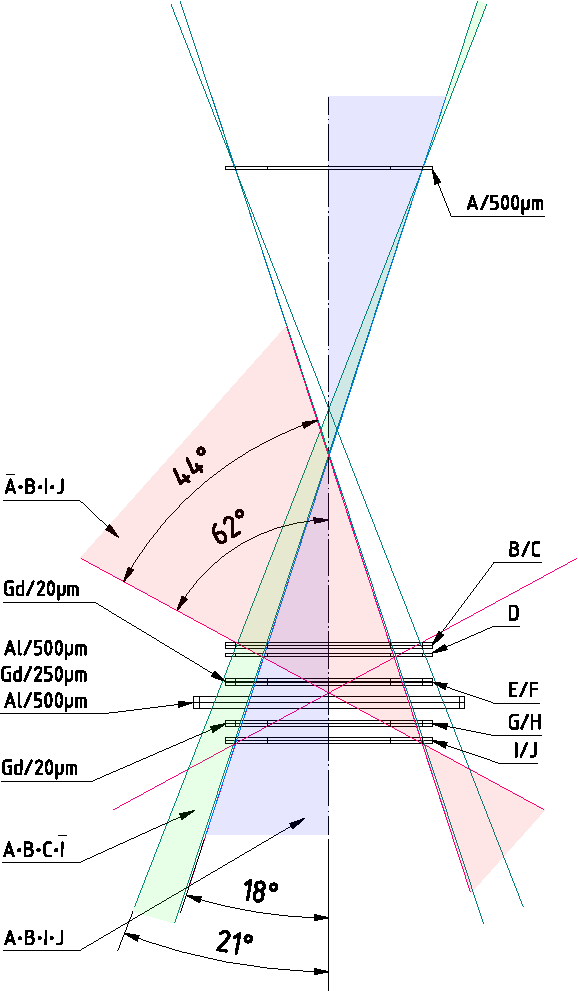
\includegraphics[width = 0.7\textwidth, height = 0.5 \textheight]{images/change4_lnd-c9_trigger-cones-colored.pdf}
    \caption[The inner structure of LND \ac{SH}]{A sketch of the inner structure of the \ac{LND} \ac{SH}. Ten 500 $\mu$m Si \acp{SSD} are assembled in order. The different colored regions indicate the \ac{FOV} of different measurement combinations. The figure was reproduced from \citet{Wimmer-2020-LND} and more details could be found in instrument paper.}
    \label{Fig:LND_sensor_head}
\end{figure}
Chang'E-4 is a robotic spacecraft mission of China exploring the lunar far-side surface, which is also the first human soft-landing missions on the lunar far-side surface \citep{Li2021SSRv}. The whole mission consists of a lander, a rover named Yutu-2 and a relay satellite named Queqiao which works in the lunar orbit and enables the communication between the lunar far-side surface and the ground. The mission was launched on December 8, 2018 and successfully landed on the Von K\`arm\`an crater near the south pole of Moon on January 3, 2019 \citep{Wu2019NatGe}. In order to cope with the significant temperature variations on the lunar surface, the rover, lander, and scientific payloads onboard enter a hibernation state during the approximately two-week-long lunar night. This mode helps to conserve energy power and to protect the detectors.  After the extended 'sleep' night, the instruments onboard are awakened by sunlight and start operating during the lunar daytime. The initial design life time of the mission was set at a minimum of one year. Obviously this target have been successfully surpassed and the scientific instruments onboard are continuing to perform impressive measurements.

As an integral part of the Chang'E-4 mission's international scientic payload, \acl{LND} is designed by the Kiel University in Germany. An image of the flight spare model of \ac{LND} is displayed in Fig.~\ref{Fig:LND_instrument}. 
The initial design purpose of \ac{LND} is to provide the first active active
dosimetric measurements and monitor the radiation environment caused by changed and neutral (neutrons and $\gamma$-ray) particles, as the preparation of future human exploration of the Moon and the solar system. Dose rate
Therefore, the main scientific objects of the \ac{LND}, as indicated in the instrument paper \citep{Wimmer-2020-LND}, are "Dosimetry for human exploration of the Moon" which is based on temporal variations of the dose rate and the \ac{LET} spectra, and "Contribution to the heliospheric science" which based on the measurement of charged particles.
% \begin{itemize}
%     \item \emph{Dosimetry for human exploration of the Moon}: \ac{LND} is designed to determine the temporal variations of the dose rate and the \ac{LET} spectra which will be used to derive the quality factor \textit{Q} which is a key factor to interprete the dosimetric data.
%     \item \emph{Contribution to the heliospheric science}: The particle fluxes and time series of the flux are measured on the far-side of the Moon. This unique measurement location provides valuable insights into the propagation of the particles in the heliosphere.
% \end{itemize}
Besides, \ac{LND} also has two technological demonstration objects which are "Determine the subsurface water content in the South-Pole Aitken Basin" and "Determine the FeO content in the South-Pole Aitken Basin" \citep{Wimmer-2020-LND}.

As of May 2023, \ac{LND} has been successfully working on the lunar far-side surface for more than 4 years, which corresponds to approximately 50 Lunar days since Jan 3, 2019. It has largely surpassed its designed lifetime.
One of the simplest way to check whether LND is working or not is to look up during the night and check the moon phase. If you can see a new moon or the moon is in the last/first quarter phase, it indicates that the moon is moving out of the earth's shadow and that the far-side surface of moon is facing the Sun, enabling the \ac{LND} work.

Based the the operations and experiment schedule established from the ground, \ac{LND} has been completely or partly (more than half a lunar day) switched off on the 6th, 44th, 45th lunar days since the start of the mission. As of the finalization of this thesis in May 2023, we have received 46 lunar days' data from January 2019 to the end of November 2022 which are stored on the servers of Kiel University. The data have officially been published in the Lunar and Planetary Data release system \footnote{\url{moon.bao.ac.cn}}, where currently the data is available until the end of December 2022. 
%you could find the data until December 2022. 
The alternative downloading options include \ac{NASA}'s Space Science Data Coordinated Archive and, \ac{ESA}'s archive ESDC (ESAC Science Data Center) which are still in building. The instrument will continue its operation on the lunar far side and we anticipate to receive more intriguing data in the future with increasing solar activities.



\subsection{LND as Charged particle telescope}

\ac{LND} has a special designed sensor head that enables it to be used as a dosimeter, neutral particles telescope and charged particle telescope. Here, we put our focus on the charged particle telescope in this section and a brief introduction to the other two components are given in the next section for a comprehensive overview of LND's capability.

The flight spare model of \ac{LND} which is an exact replica of the flight model currently deployed on the moon is displayed in Fig.\ref{Fig:LND_instrument}. The instrument is composed of two seperate parts, the \acl{SH} in the front and the \acl{EB} at the rear. \ac{SH} and \ac{EB} are connected by a 1-meter cable which serves to provide power and transfer data. 
The \ac{SH} is comprised of ten segemented Si \acs{SSD} of norminal 500 $\mu$m thickness. They are labeled from A to J and assembled in a charged-particle telescope configuration as illustrated in Fig.~\ref{Fig:LND_sensor_head}.

The structure of the telescope can be further divided into two parts. The upper half consists of four detectors (A, B, C, D) with A placed 80.5 mm away from B. The detector A is crucial for the function of \ac{LND} as charged particle telescope since only particles that trigger detector A will be counted. B/C/D are assembled as close in space as possible, with zero space between B and C and 0.5 mm between C and D, enabling the anti-coincidence measuremet in the inner C segement. Such a detector arrangement is similar to the Flight Radiation Environment Detector (FRED) \citep{moeller-etal-2013, moeller-etal-2013b}. The lower half consists of three detector pairs (E/F, G/H, I/J) and an Al-Gd-Al absorber. The detector pairs are closely packed together and the absorber is designed for the detection of thermal neutrons. 20 $\mu$m thick Gd foils are inserted into E/F and G/H, creating sandwich-like structures to detect thermal neutrons. This charged particle telescope is completed by the last detector pair I/J.

By measuring the energy depostion in different \acp{SSD} and using the dE/dX - E or dE/dX - dE/dX methods which depend on the primary energy of particles, LND can easily identify the energies and species of particles. 
The averaged energy loss of the charged particle along the travel path depends on the nuclear charge $Z_1$ (equal to atomic number) and the incident velocity $\nu$. 
Such a relationship could be expressed by the well-known Bethe-Bloch formula \citep{bethe-1930, bloch-1933}:

\begin{equation}
    \frac{\dd E}{\dd x} = - \frac{Z_1^2 e^4 n_e}{4 \pi \cdot \varepsilon_0^2 \beta^2 c^2 m_e} \cdot \left[ \ln\left(\frac{2 m_e  \beta^2 c^2}{{E_B}}\right) - \ln(1 - \beta^2) - \beta^2  \right], 
    \label{eq:BB}
  \end{equation}
where $c$ is the speed of light, $\beta = \nu/c$, $E_B$ is the ionization energy of the medium that particle pass, and $n_e$ is the electron density in the medium, $m_e$ is the electron mass, and constant $\epsilon_0$ is the permittivity of free space. $E$ is the energy of the particle and $x$ is the travel length of the particle in the medium.

The expressions in the square brackets simplifies to $ln(\beta^2)$ plus an extra constant. Because $ln(\beta^2)$ is nearly constant and slowly changes in the energy range coverd by \ac{LND}, therefore the above equation could further simplifies to:
\begin{equation}
    E_A \propto \frac{Z_1^2 m_1}{E_{\mathrm tot}},
    \label{eq:BB2}
\end{equation}
where $E_A$ is the energy loss in the detector A, $E_{\mathrm tot}$ is in principle the primany energy of particles.
The product of $E_A$ and $E_{tot}$ is proportional to the square of nuclear charge, $Z_1^2$ which equals to the atomic number and the mass of elements, $m_1$. These parameters depend on the particle species and allow for the determination of particle compositions. It is worth noting that \ac{LND} has the capability to discriminate between the isotopes of elements, such as helium-3 and helium-4, despite the limited resolution and larger uncertainty. See Appendix \ref{chp:appendix_LND_He3_spectra} for more details.

%The nuclear charge $Z_1$ is equal to the number of protons in the nucleus, i.e. the atomic number $Z$ of the elements. Therefore, the telescope like \ac{LND} can not determine the particle charge state and we could not tell apart fully charged \ac{GCR} and singly charged \ac{ACR}. When traversing the front foil and \acp{SSD} of \ac{LND} sensor head, those partially charged particle will be ionized and stripped the electrons, becoming fully charged \citet{Swaczyna2017ApJ}.


Once the charged particle enter the sensor head of \ac{LND}, they can be further categorized into two groups: stopping particles and penetrating particles. Stopping particles have a primary energy range between $\sim$ 8 MeV/nuc and $\sim$ 35 MeV/nuc, stopping within any of the detectors B-I. Penetrating particles possess energy above this range and have the capability to penetrate through all the detectors. In Fig.~\ref{Fig:LND-Boehm-plot}, a plot generated by the large counting statistic \ac{Geant4} \citep{Agostinelli-2003} simulation illustrates how the stopping particles are seperated by using $E_{tot} * E_A$ as the y-axis and $E_{tot} / E_A$ as the x-axis. 
Notely, due to the thick absorbers in the middle of detector stack, the total energies of particle that stop in detectors F to I are unknown. Therefore, we use the summation of energy deposition in detectors A to D as the $E_tot$ above (See table 5 of \citet{Wimmer2020SSRv}).
The data points are simulated in \ac{Geant4} based on a carefully construced \ac{LND} instrument model. This model takes into account all the inner structures within the sensor head, including the \ac{PCB} next to the detector stacks and the outer shell of the sensor head. However, we must note that a completed model including the surrounding material of \ac{LND} is unavaiable since we lack the structure information of the Chang\'E-4 lander.
A screenshot of the \ac{LND} model is provided in the appendix \ref{chp:LNDsimulation}, presenting the detailed structure of the \ac{LND} sensor head.

Penetrating particles have a primary energy above approximately 35 MeV/nuc, and as the name suggested, can penetrate through detectors A to I and stop in J or continue to penetrate J with more energy. The majority of the penetrating particles are fully penetrating particles, which means we can not directly measure their total energy. 
%\acp{MIP} are among the fully penetrating particles that have extremely large initial energy from hundreds MeV to GeV but only deposit a minimal amount of energy in the detector stacks.
Since the total energy of particles is unavaiable, it is not possible to create a plot similar to Fig.~\ref{Fig:LND-Boehm-plot}. Instead, we change the formula of x-axis and y-axis to $E_I/E_A$ and $dE$ respectively. The $E_I$ is the energy deposit in the last detector I. The $dE$ is the energy deposition summed from the B, C, and D.

Notably the incident direction of the particle i.e. whether they come from above or beneath the detector, could be inferred from the penetrating data. From the Bethe-Bloch formula, we figure out that the energy loss of a particle decreases with the increase of the incident energy. 
Therefore, the particle that incidents from above deposites less energy in the front detector A than the bottom detector I and the ratio $E_I/E_A$ tends to be larger than 1. While for the particle entering from beneath, more energy deposition in detector A than that in detector I, hence the ratio tends to be less than 1. 
By analyzing the distributions and patterns in the histogram, we can identify the albedo protons from the 2-D histogram of penetrating particles, corresponding to columns 248 - 264 of Fig.~\ref{Fig:measurement_Xmas}.
The detailed understanding of the derivations and analysis of albedo protons could be inferred from Section. ~\ref{chp:LND_GCR_albedo}


\begin{figure}
    \centering
    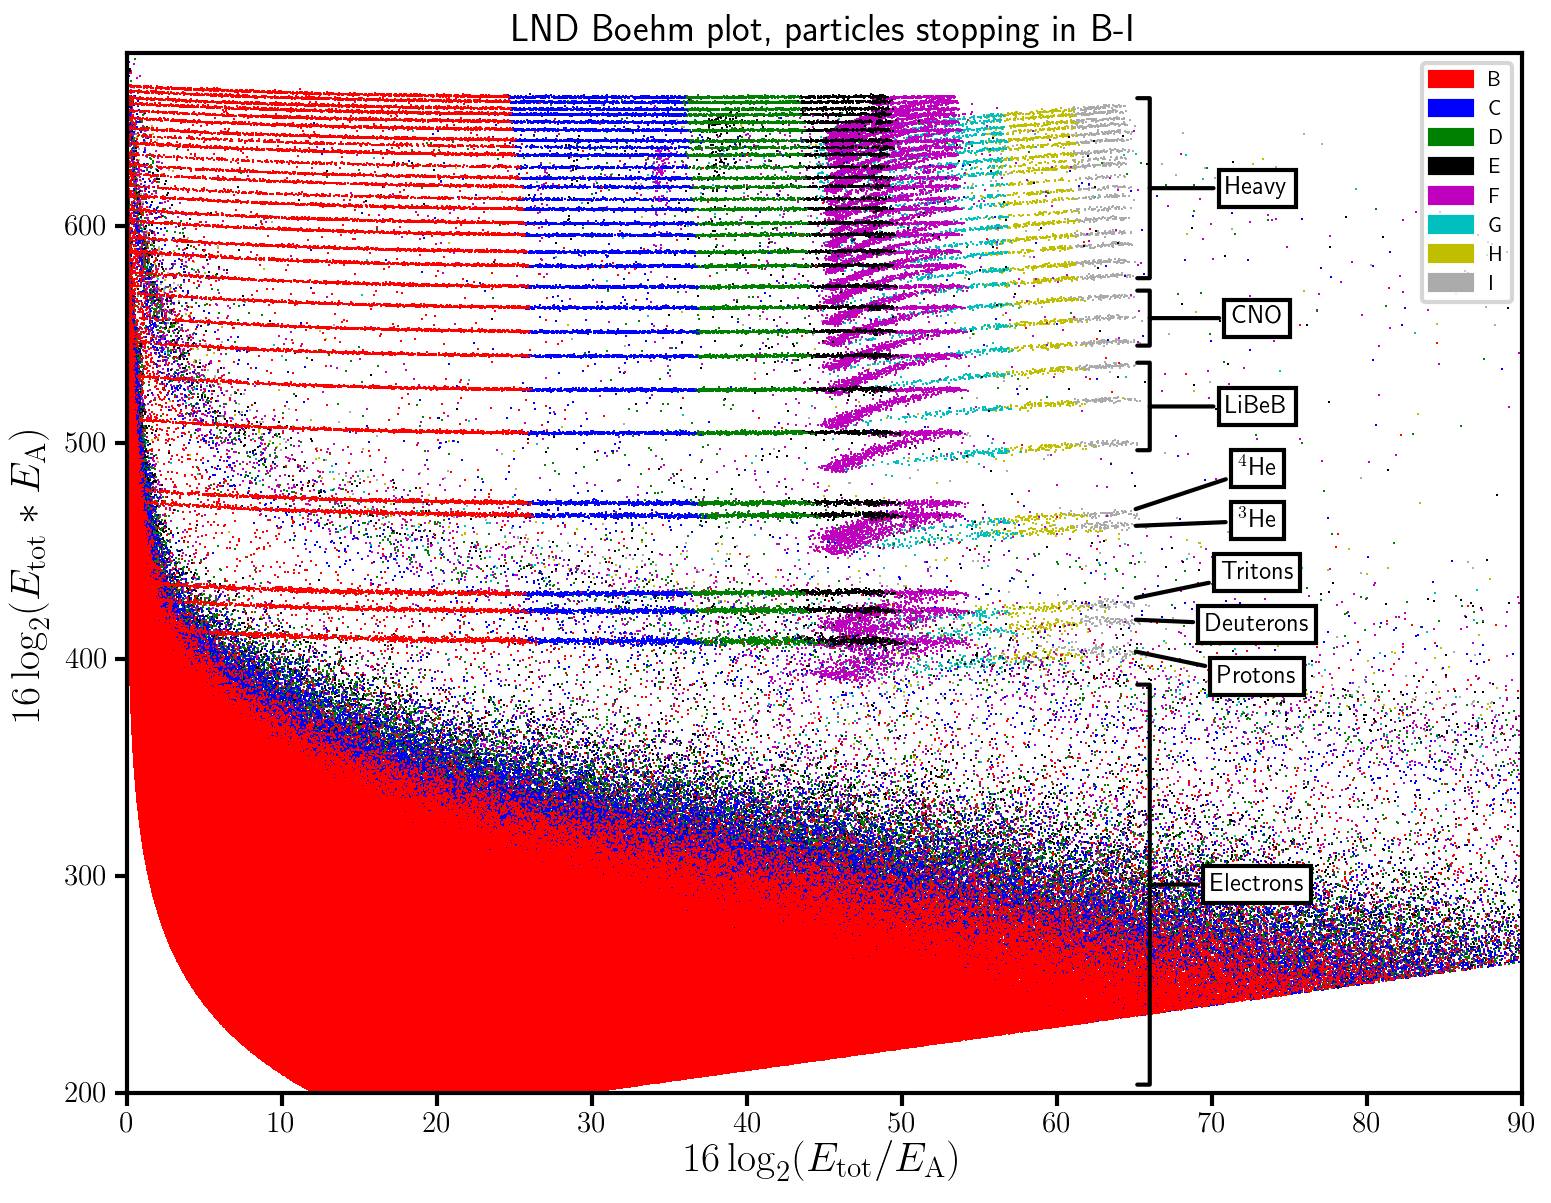
\includegraphics[width=0.8\textwidth]{images/LND_Boehm_plot_isotropic_on_top_of_A_annotated.png}
    \caption[LND Boehm plot of stopping particles based on the simulated data]{The different particle species are well discriminated in this LND Boehm plot which is a scatter plot of the \ac{LND} simulation data generated by the \ac{Geant4} tools \citep{Agostinelli-2003}. During the simulation, an isotropic source is positioned above detector A.}
    \label{Fig:LND-Boehm-plot}
\end{figure}


\subsection{LND as dosimeter and neutral telescope}

\ac{LND} measures the \ac{TID} in the inner B segment utilizing the energy deposition and corresponding energy spectrum. The inner segment of C, which is surrouded by the B, D and C outer segment and in anti-coincidence with all other detector segments, is used to measure the neutral dose rate caused by both fast neutrons and $\gamma$-rays. The above two measurements are the primary data products of \ac{LND}. \ac{TID} and dose in C play important roles in assessing the radiation environment on the lunar surface. 

\ac{LND} employs the E/F, G/H pairs which clamp a Gd-foil, to measure the thermal neutron flux. The Gd-foil has a large cross section for thermal neutrons, resulting in an increased possibility of interaction with those neutrons \citep{Wimmer2020SSRv}. After the capture of thermal neutrons in the Gd-foil, x-ray with energies of 43 keV and electrons with energies of 71 keV, 131 keV, and 173 keV are emitted and then detected by detectors closed to the foil.
In the calibration experiment, \ac{LND} successfully measured neutrons by calculating the energy spectrum discrepancy between E (G) and F (H) for neutrons coming from the front (back).
However, in real measurements, the quality of the thermal neutron data is unexpectedly low due to various factors. The most prominent factors is the neutron background emitted from the \ac{RTG} and the \ac{RHU}. These radioactive sources generate heat to protect the lander and payload from the frozen night. But they also contribute largerly on the neutron background \citep{Zhang2020SciAdv}. Unfortunately, the direct measurement of the radiaion sources had never been done, and only an experimental and empirical estimation of the contamination from the background on the data were conducted by \citet{Hou2020-LNDbackground}. Based on data from laboratory experiements and Monte-carlo simulations, \citet{Hou2020-LNDbackground} confirmed the non-negligible background interference and firstly estimated the dose rate background. 

Another factor that might affect the neutron measurements is the unanticipated noise increase in these detectors. Similar to the noise issue occured in other channels, channels F2, G2 and H1 have also been troubled by an increased noise level (further discussed in Section \ref{chp:LND_GCR_albedo}). The single detector counter rates increase from $10^3$ count/min to $10^6$ count/min and energy spectra of noise channels indicate that the dominant energy is below 300 keV.
The high energy noise obscure the x-ray line at 43 keV and electron lines at 71 keV, 131 keV, and 173 keV which are used to determine the thermal neutrons flux, and make it more challenging to derive the accurate thermal neutron flux of lower intensity.
Furthermore, increased number of noise in those thermal neutron channels cause serious dead time issues on the data product neutron dose in C. This is because neutron measurements share the same counter buffer. The dose in C is the primary objective of \ac{LND}. In order to mitigate the dead time issue, we raise the corresponding threshold of noise detectors to few hundreds keV (depending on the noise level of each detector), resulting in the loss of the thermal neutrons data.


The remain data products related to the radiation are the \ac{LET} spectra. \ac{LND} provides three types of \ac{LET} spectra including \ac{LET} $ABC\bar{I}$, $\bar{A}BIJ$ and $ABIJ$. Those \ac{LET} spectra can be used to derived the quality factor (Q), which multiplies the absorbed dose rate to obtain the dose equivalent.
Of note is that geometry factors of these \ac{LET} spectra are also affected by the configuration changes. We provide the changes of geometry factors in the appendix of chapter \ref{chp:LND_GCR_albedo}.
%More details of the data products can be found in the instrument paper \citet{Wimmer2020SSRv}.

The first scientific result of \ac{LND} regarding the radiation environment on the lunar surface are reported in \citep{Zhang-2020-LND-firstresults}. These initial findings present the \ac{TID}, neutron dose and \ac{LET} spectra of the first two lunar days. This represents the first ever dynamic measurements of the radiation variation on the lunar surface. The averaged total absorbed dose rate in silicon is about 13.59$\pm$1.01 $\mu$Gy/hour. Amongst this total dose rate, the contribution from neutral particles is estimated to be $3.10 \pm 0.43 \mu$Gy/hour. These values are consistent with the measurements from the \ac{CRaTER} on \ac{LRO}.



\subsection{Primary data products: Xmas plots}
\label{sec:xmas}

\begin{figure}
    \centering
    \includegraphics[width =0.95\textheight, height = 0.4\textheight, angle = 90]{images/xmas-2019-01-03To2022-11-29.png}
    \caption[\ac{LND} Xmas plot from measurements]{The completed Xmas plot (274 $\times$ 64) of \ac{LND} based on the measurements between 2019.1.3 and 2022.11.29. All the data products could be found in this matrix, including neutrals, \ac{LET} spectra, \ac{TID}, stopping and penetrating charged particles, including electrons, protons, helium nuclei and heavy ions. The corresponding simulation version can be found in \citep{Wimmer2020SSRv}}
    \label{Fig:measurement_Xmas}
\end{figure}

Fig.~\ref{Fig:measurement_Xmas} is the so-called "Xmas plot" \footnote{It was the front cover of the Xmas card of IEAP group in 2017. Hence we named it Xmas plot} of the \ac{LND}.The Xmas plot is an image of \ac{LND}'s memory space shaped in a 274 $\times$ 64 matrix, where each pixel in the Xmas plot servers as a counter. In principle all data products are extracted from this matrix. 
When \ac{LND} detects the deposited energy in detectors of an effective signal, the control units will calculate onboard the appropriate position in the Xmas plot and increment the corresponding counter. 

Unlike the simulated plot in \citep{Wimmer2020SSRv}, here we showcase an Xmas plot from the actual measurements between 2019.1.3 to 2022.11.29, encompassing all the data accumulated since the first lunar day observed by \ac{LND}. The green rows are the memory space that will not be transmitted to the ground, in order to save the telemetry bandwidth. 
For a more detailed explanation of the format of the Xmas plot, I recommend \citep{Wimmer2020SSRv}.


\ac{LND} measures and provides the data products including up to 1-minute charged and neutral particle dose rate measured in Si, up to 1-minute cadence \ac{LET} spectra, 1-minute neutral particle deposition energy spectra, 10-minutes count rates of thermal neutrons and high time resolution (1-minutes, 10-minutes) charged particles flux and high energy resolution spectra including electrons and ions from proton to iron.

%The major different compared with the Xmas plot in \citep{Wimmer2020SSRv} is that LND measure not only the particle incident from above but also the albedo particles moving upward, while in the simulation, we did add the albedo component. It is obvious that in the penetrating panel of Xmas plot,  a higher than backgrond branch strech from middle to the left side. This branch represents the protons moving upward with enough energy fully penetrating all the detectors as well as the extra shielding from the lander structure. More details of how to derive albedo proton flux are given in Section.~\ref{sec:albedo_proton}.

\subsection{Configuration changes of LND}

It is important to highlight that several configuration changes have been implemented after \ac{LND} was delivered and launched. Those configuration changes are reflected in 14 extra commands, which are uploaded to the control unit of \ac{LND} every morning of lunar day, fixing software issues and malfunction issues. One of the software issues arises from errors in the software pipeline where the control unit use wrong channels to determine particle energies. Another one is due to the mistakes we made in simulations when designing data products, causing location of the \ac{dps} boxes shift in the X-mas plot which is a matrix storing \ac{LND} data products (See below and \citet{Wimmer-2020-LND} for more details about the X-mas plot). Neverthless, the impact of the second problem on the data products is minor. 

The significant changes of the data products are mainly caused by raising the threshold of noise channels and by removing the A2 channel in the level 3 trigger logic. A2 represents the outer segement of the front detector A (see Appendix in Sec.~\ref{chp:LND_GCR_albedo} for more details of the changes). These changes are motivated by high observed noise levels in detectors A, G, H, I and J which appeared coincidentally with the malfunction of the front lid. The front lid of \ac{LND} is a part of the lander and is designed to protect the fragile detectors inside the \ac{SH}. The lid is opened up to allow unobstructed measurements of the particles during lunar days, and is closed immediately after the instrument is switched off, protecting the detectors from the extreme temperature dercrease on the lunar surface and the lunar night. However, on the 3rd and 4th lunar day, \ac{LND} was switched off for a short period during working time but the lid was left open. Though temperature on the lunar surface increased as the Sun rose, \ac{LND} and its detectors kept losing heat. Hence the temperature of the \ac{SH} dropped drastically, resulting in irreversible deformation of carriers and the attached detectors, particularly the detectors A and I/J in the front side and the bottom side. Consequently, the lower energy noise ($\sim$ 10 - 200 keV) experienced a significant increase.

By implemmenting the aforementioned changes, we have sucessfully reduced the noise level and mitigated its impact on the primary data products such as \ac{LET} spectra. However, it is worth noting that these changes still resulted in significant consequences for several data products. For instance, we partly lose the measurement of \acp{MIP} after the increment of the threshold of I detector; the geometry factors of two \ac{LET} spectra and penetrating particle are reduced dramatically after disabling the A2 channel, which plays a key role in \ac{LND}'s measurement logic. For a better understanding of the configuration changes and their impact on the data products, please refer to the appendix of chapter \ref{chp:LND_GCR_albedo}.
The corresponding changes of the original code in the LND data processing pipeline is given in the appendix ~\ref{chp:appendix_LND_data_process_pipeline}.

\section{Solar orbiter and High energy telescope}
\label{sec:Solar_Orbiter}
Successfully launched on Feb 10, 2020, \ac{SolO} mission \citep{Mueller-2020-SolO} is an international mission cooperated between \ac{ESA} and \ac{NASA} with the aim to understand the Sun and how it controls the helisphere. As indicated in the mission paper, the following scientific questions will be answered and further studied: (a). What drives the solar wind and where dose the coronal magnetic field originate from? (b). How do solar transients drive heliospheric variability? (c). How do solar eruptions produce the energetic particle radiation that fills the heliosphere? (d). How does the solar dynamo work and drive connections between the Sun and the heliosphere?

%After finishing the cuise phase which started at June 14, 2020, \ac{SolO} has been operating in the nominla mission phase since Nov 26, 2021 as scheduled.

\ac{SolO} has an elliptic helioscentric orbit with the closest perihelion of 0.29 AU (about 42$\times10^6$ km). Using several gravity assist maneuvers during the Venus flybys and the Earth flybys, the orbit of \ac{SolO} will gradually tilt away from the ecliptic plane and in the end can be 24 degrees above the Sun's equator. As of May 2023 \ac{SolO} is still following an elliptical orbit circling the sun, with a maximum solar latitude of 8.66 degrees. \ac{SolO} has finished 5 perihelions with a closest distance of 0.292 AU on Sep 3, 2022, and has started its 6th orbit, moving away the Sun. Benefiting from the unique position of \ac{SolO} during this trip, the multiple scientific instruments onboard the \ac{SolO} could further advanced our understanding of the Sun and its effects on the heliosphere.
%Three time Venus flyby happened on Dec 27, 2020,  Aug 9, 2021 and Sep 4, 2022. The Earth GAM happend on Now 27, 2021.
%The above mentioned solo tragjectory information is taken from the Solar orbiter Consolidated Report on Mission analysis \footnotes{\url{https://issues.cosmos.esa.int/solarorbiterwiki/display/SOSP/Trajectory+Overview+-+10+February+2020+Launch}}

%in the relative field for instance the questions regarding solar coronal, solar magnetic field, solar wind, \ac{SEP}.
The \ac{EPD} \citep{RodriguezPacheco-2019-EPD} is part of the scientific payload onboard \ac{SolO}, measuring energetic particles over a large scale from few kev to GeV. The spectra, composition, time variations and directional distributions could be obtained and derived.
\ac{EPD} is comprises of four different sensors, the \ac{SIS}, the \ac{STEP}, the \ac{EPT} and the \ac{HET}. 
\ac{SIS} is a time-of-flight mass spectrometer that measures ion composition from $\sim$ 0.1 - few MeV nucleon$^{-1}$. \ac{STEP} measures electrons and ions with lower energies between 4 keV and 80 keV. The special design of \ac{STEP} allows it to have high pitch-angle resolution.
\ac{EPT} and \ac{HET} share the same electronics and they are composed of two identical sensor units that are assembled perpendicularly on \ac{SolO}. This configuration enables detection of the particle incident from four different directions. \ac{EPT} is designed to measure medium-energy electrons and ions within the energy range of 25 keV to 400 keV ($\sim$ 6 MeV for protons), while \ac{HET} completes the higher energy end, measuring electrons from 300 keV to 30 MeV and ions from 6.8 Mev/nuc to $\sim$ 100 MeV/nuc in the nominal data products. Notably, the penetrating data products of \ac{HET} could extend the energy coverage of \ac{HET} up to $\sim$ GeV/nuc \citep{Elftmann-2020-PhD}.
The completed energy coverage of those four instruments for different particle species are given in Fig.~\ref{Fig:EPD-energy-coverage}.
In this section, we provide a brief introduction of \ac{HET}, which is the focus of the study in Section \ref{chp:ACR_Helium}. Further more detailed information on the other components can be found in the instrument paper \citep{RodriguezPacheco-2019-EPD} and the first years overview paper from \citet{Wimmer2021AA}.


\begin{figure}
    \centering
    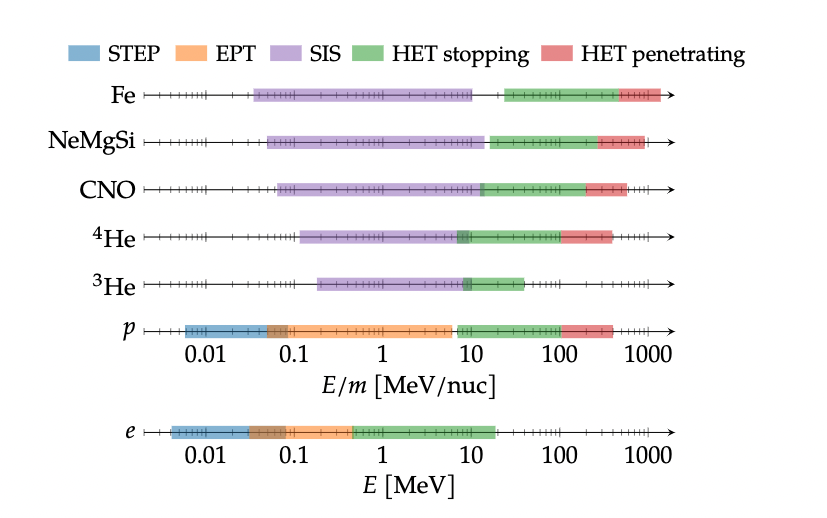
\includegraphics[width = \textwidth]{images/EPD_coverage.png}
    \caption[The energy coverage of \ac{EPD} instruments]{The energy coverage of different \ac{EPD} instruments for different particle species. This figure is an updated energy coverage plot made by \citep{JohanPhd2020}, based on the similar plot from \citep{RodriguezPacheco-2019-EPD}. The HET measurements are split into stopping and penetrating parts and the later one can largely extend \ac{HET}'s capability \citep{Elftmann-2020-PhD}.}
    \label{Fig:EPD-energy-coverage}
\end{figure}  

\subsection{High energy telescope}

\begin{figure}
    \centering
    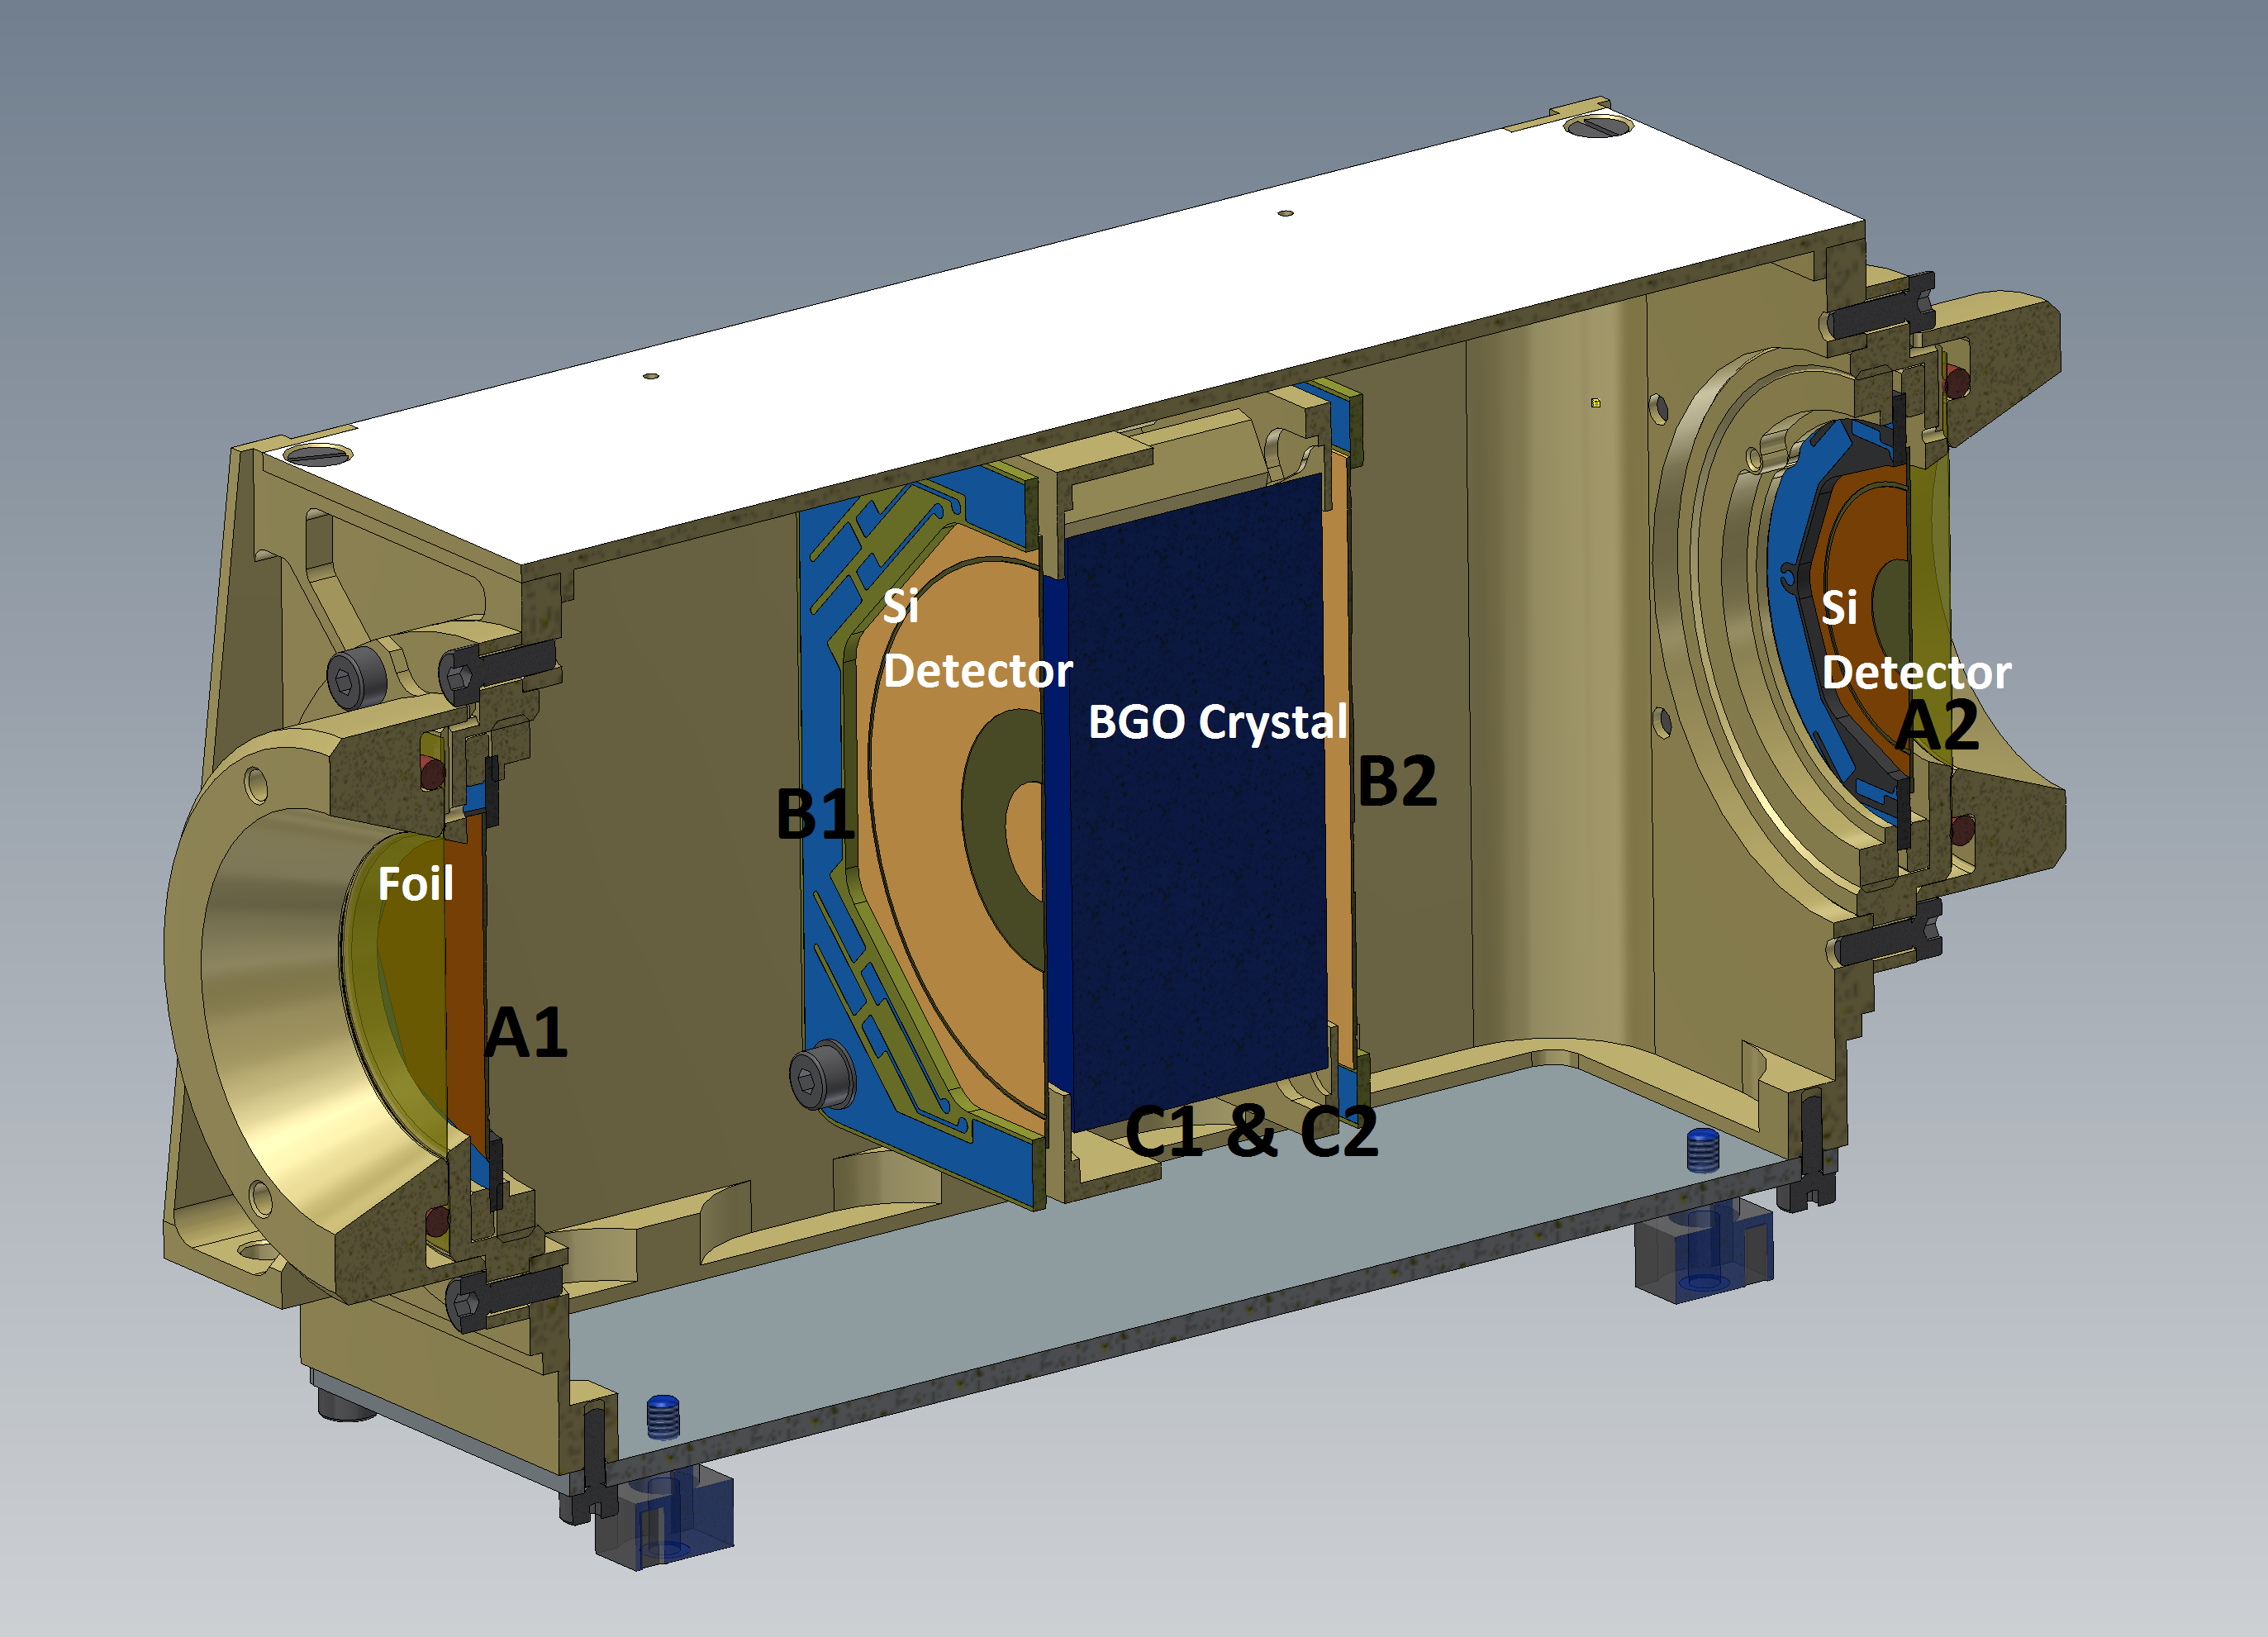
\includegraphics[width = \textwidth]{images/het.png}
    \caption[The \ac{HET} sensor head]{The cross profile of the \ac{HET} sensor head. The detector names are labeled. Figure is reproduced from \citet{RodriguezPacheco-2019-EPD}.}
    \label{fig:HET-sensor-head}
\end{figure}

\ac{HET} is a double-ended telescope. The cross profile of the \ac{HET} sensor head is depicted in Fig.~\ref{fig:HET-sensor-head}. The sensor head of \ac{HET} consists of four 300 $\mu$m silicon \ac{SSD} stacks, with two in each side (A1, B1 in the front side and A2, B2 in the back side), and a 2-cm thickness \ac{BGO} ($Bi_{4}Ge_{3}O_{12}$) scintillator which is named as detector C in the center. The sensor head setup is similar to the configuration of the \ac{RAD}, another instrument developed by Kiel Univeristy, which is currently operating on the Martion surface.  

\ac{HET} uses the $\mathrm{dE/dX - E}$ technique to discriminate different particle species of different energy. This method is the same as the measurement principle of \ac{LND} that has been well explained before. The particle species that \ac{LND} can discriminate include electrons, protons, helium nucleus, and all heavy ions such as carbon, nitrogen, oxygen, and iron.  

Once the charged particle incident and penetrate the A detector (A1 or A2), they can be split into stopping particles and penetrating particles, depending on their energy and whether they stop in detector B/C. As given in Table 22 of \citet{RodriguezPacheco-2019-EPD}, the corresponding nominal data products are ABnC, which is corresponding to particles stopping in B with energy of 6.5 - 9.5 Me/nuc, ABC which register particles stopping in C with energy range of $\sim$10 - $\sim$ 100 MeV/nuc, and penetrating detector C with energy above 100 MeV/nuc up to infinity. 

%For the penetrating particle, their primary energy can be estimated based on the energy loss on the detector and the \ac{Geant4} simulation. The aforementioned nominal data products of HET contribute to the study of \ac{SEP}, \ac{ACR} and \ac{GCR}.


In addition to the nominal charged particle data products, it is important to emphasize the significant contribution of housekeeping data in our studies.
The housekeeping data are \ac{EPD} sensor produced instrumental data. They have the highest priority for downlink to the Earth and are used to monitor the instrument status and health. Although the housekeeping data are not designed for scientific purpose, they still provide valuable insight into the instrument performance and their contributions to the scientific studies is impressive \citep{Wimmer2021AA}.


Such a housekeeping data is the single detector counter which register signals in the \ac{BGO} scintillator crystal, this is the C detector. This counter does not require any coincidence condition and respond to particles from all directions and types. The sole requirement is that the deposited energy exceeds the threshold of the C detector. Due to its larger geometry factor, this counter exhibits better counting statistics and can be used to detect small disturbance in the \ac{GCR} background. For example \citet{Forstner-2021-SolO} use this counter to study a \ac{FD} with an ampliude of 3\% when a \ac{CME} passed \ac{SolO} on 19 April 2020. In addition, \citet{Allen2021AA_venus} found an $\sim$ 5\% drop in the count rates during the first Venus flyby. This drop is due to the planet body blockage on the \ac{FOV} of \ac{HET}.

Similar to the single detector count rate, we also utilize the L2 counters named \textit{any(a1, b1)} or \textit{any(a2,b2)} to determine the periods of \acp{SEP}. The counters sum up every signal that triggers detectors A1 (A2) and B1 (B2) in the sensor head, regardless of the primary energy and the particle species. \acp{GCR} which are slowly varying are the dominant particles in the background of this counter. Therefore, a temporal increase indicates an incoming of \ac{SEP} event. These data products exhibit better counting statistics than the nominal science data products which are designed to derive the flux. Additionally, \textit{any(a1, b1)} or \textit{any(a2,b2)} are more sensitive to lower energy particles from \acp{SEP}, as they have a lower energy threshold of $\sim$ 50 keV compared to the C counter \citep{Elftmann-2020-PhD}. The counters can detect electrons and ions with energy below 1 MeV. As a result, those two counters are particularly useful in determining the start and end time of the \ac{SEP} events, no matter what particles trigger them. In Section~\ref{chp:ACR_Helium}, where we are interested in \acp{ACR}, we remove \ac{SEP} time periods determined by this method based on the \textit{any(a1,b1)} counter to enable an accurate \ac{ACR} measurement.


For more details on the inner structure and parameters of the \ac{HET}, as well as the most update status of \ac{HET}, one could refer to \citet{RodriguezPacheco-2019-EPD, Wimmer2021AA,Elftmann-2020-PhD}.

